\documentclass[crop,tikz,border=2px]{standalone}
\usepackage{tikzsymbols}
\usetikzlibrary{arrows,positioning,scopes}
\begin{document}
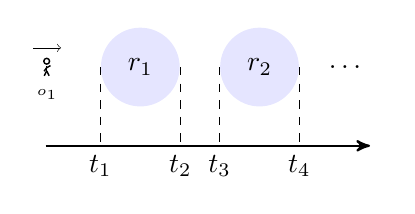
\begin{tikzpicture}[
  reader/.style={circle,minimum width=1cm,fill=blue!10,node distance=.5cm},
  timeline/.style={->,>=stealth',thick,shorten <=2pt,shorten >=2pt}]

  \node[reader] (r1) {\(r_1\)};
  \node[reader] (r2) [right=of r1] {\(r_2\)};
  \node[reader,fill=none] (r3) [right=.1cm of r2] {\ldots};

  \node[below=1cm of r1.west] (t1) {\(t_1\)};
  \node[below=1cm of r1.east] (t2) {\(t_2\)};
  \node[below=1cm of r2.west] (t3) {\(t_3\)};
  \node[below=1cm of r2.east] (t4) {\(t_4\)};

  \path[timeline,draw] ([xshift=-.5cm]t1.north west) -- ([xshift=.7cm]t4.north east);

  \draw[very thin,dashed] (r1.west) -- (t1);
  \draw[very thin,dashed] (r1.east) -- (t2);
  \draw[very thin,dashed] (r2.west) -- (t3);
  \draw[very thin,dashed] (r2.east) -- (t4);

  \node[left=.5cm of r1] (obj) {\Strichmaxerl[][54][28]};
  \draw[->,very thin] (obj.north west) -- (obj.north east);
  \node at ([yshift=-1mm]obj.south) {{\tiny \(o_1\)}};
\end{tikzpicture}
\end{document}